\section{Evaluation}
\label{sec:evaluation}
% \meiyi{make sure we update all results if the data change}
% TO-DO Data
% \begin{itemize}
%     \item data sets (rom, stab., external rotation)
%     \item metrics?
%     \item baseline
% \end{itemize}
% TO-DO
% \begin{itemize}
%     \item Baseline of PCA does not do well on classification
%     \item modular MLP classification of ROM
%     \item modular MLP classification of stability (binary or not?)
%     \item modular Siamese network of difference of two ROM of the same user
%     \item 
% \end{itemize}



% [TODO summary of Evaluation]

We evaluate PhysiQ from three perspectives: model performance in exercises, generalizability in different metrics, and importance of components in the model. We compare the overall performance of the framework with different types of baseline and how the model performs in different exercises and metrics. We explain the design and set up in Section  \ref{evaluation:subsec:implementation}, \ref{evaluation:subsec:traintest}. Additionally, we test our model performance and generalizability in Section  \ref{evaluation:subsec:performance}. Lastly, we evaluate our model's components in Section  \ref{evaluation:subsec:parameters} and Section  \ref{evaluation:subsec:ablation}. 
% One of the goals of this paper is to see if our model reduces the dependency on expert knowledge for the engineering process that professionals have to work on. If the models can understand our metrics, we can have therapeutic knowledge to build much more advanced metrics for the model to learn.
\subsection{Implementation}\label{evaluation:subsec:implementation}
We implement the PhysiQ application in consumer-level IOS Apple Watch with an automatically connected application on iPhone. PhysiQ uses a built-in accelerometer and gyroscope to collect sensory motion data and analyze the data quantitatively. The maximum sampling rate that we choose is 50 Hz, because through our analysis of a single exercise, we observed that the Fourier frequency is mostly below 10 Hz, and other papers also support this observation \cite{HUMAN_MOTION_FREQUENCY_2013}. Additionally, one of our metrics is stability, and such core motion of the body should be captured more cautiously with a higher frequency rate. Thus, 50 Hz is what we decide to use. Lastly, once the users have performed exercises, the result automatically synced from the watch to the smartphone through Xcode WCSessions. 

\subsection{Training and Testing Dataset}\label{evaluation:subsec:traintest}
Once the data is recorded, we segment the data according to our energy function. We used weights $W_x$,$W_y$,$W_z$ for each accelerometer x, y, and z, and $\lambda$ as an additional hyper-parameter. Next, we split the dataset and apply standard scales for all exercise segments; the scaler is an axis-wise scaler standardized on the current axes (x, y, and z for both accelerometer and gyroscope sensory data). There are two splitting methods for evaluation we employed. The first one is leave-one-person-out cross-validation (LOOCV). LOOCV is a cross-validation approach that treats each subject as a “test” set. This type of k-fold cross-validation has the k value as the number of participants. LOOCV separates the models from seeing the validation/testing set. As a result, the model does not see the distribution of validation subjects (participants), and we can analyze the generalizability of our model on 34,000 training samples and about 3,000 validating and testing samples, of total 31 participants. In ROM and stability, we have a total of 37000 data samples. In repetition, we perform a repetition comparison among 1, 2, and 3 repetitions, with a total of 280,000 data samples in shoulder abduction, 15,000 in external rotation, and 8,000 in forward flexion. For efficiency, we randomly choose 10\% of the data in shoulder abduction for the overall evaluation 10 times. Secondly, we perform a standard 70\% 10\%, and 20\% respectively on training, validation, and testing splits as our overall evaluation. We randomly extract these splits in each subject in 70, 10, and 20 fashions in normal splits. By having both evaluations, we should know how our model works in real-world scenarios and how well our model can perform. 

% \begin{table}[h!]
% \centering
% \begin{tabular}{||c c c c c||} 
%  \hline
%  & PhysiQ & RNN & SimCLR & VGG \\ [0.5ex] 
%  \hline\hline
%  MSE &       0.00280107 & 0.0289637 & 0.0104795   & 0.0469153\\ 
%  MAE &       0.0432687    & 0.133548 &  0.0785231      & 0.179209 \\
%  R-squared & 0.932884   & 0.305932 & 0.757808       & -0.0817496\\
%  \hline
% \end{tabular}
% \caption{TODO: Average results for overall evaluation}
% \label{table:normalTraining}
% \end{table}

\subsection{Evaluation Metrics}\label{evaluation:subsec:evaluationmetrics}
We evaluate the performance using three measure methods in all experiments, i.e., R-squared, Mean Square Error (MSE), and Mean Absolute Error (MAE). R-squared, the coefficient of determination, is how close the data are fitted in the model or the percent of variation explained by the model. MSE measures the mean of the squares of the errors, meaning it calculates the average squared difference between predicted and target values. Finally, MAE measures how far predicted values are from observed values with their absolute difference. Equations shown below:
\begin{equation}
    R^2 = 1- \frac{\sum_i(y_{i} - \hat{y_i})}{\sum_i(y_{i} - \bar{y})},
\end{equation}

\begin{equation}
    MSE = \sum_{i=1}^n(y_{i} - \hat{y_i})^2,
\end{equation}

\begin{equation}
    MAE = \frac{\sum_{i=1}^n|y_{i} - \hat{y_i}|}{n},
\end{equation}
where $n$ is the number of dataset, $\hat{y_i}$ is the predicted value, $y_i$ is the ground truth value, and $\bar{y}$ is the mean value. $\hat{y_i}$, in our case, is the similarity score of two inputs of segments, and $y_i$ is our ground truth of similarity score based on \textit{range of motion}, \textit{stability}, or \textit{repetition}.
 To test our model with the baselines, we evaluate the experiments on our local machine with a CPU of AMD Ryzen 9 5950X with a 16-Core processor (3.40 GHz), RAMs of 64 GB (3200 MHz), and a GPU of Nvidia GeForce RTX 3090. The operating system is Windows 10 Pro. Additionally, we envision to deploy our deep learning model into cloud server to support API call directly from our mobile application.

\subsection{Performance}\label{evaluation:subsec:performance}

\subsubsection{Siamese Similarity}
We explore different ways of quantitatively measuring our exercise metrics. There are two necessary baseline models: RNN and CNN because RNN is known for arbitrary input with time-varied data, and CNN learns well in spatial and temporal features \cite{stromback2020mm}. Additionally, we choose SimCLR as third baseline because its architecture enables useful representation learning in contrastive learning \cite{SIMCLR2020}. Thus, we provide and twist the networks such as SimCLR \cite{SIMCLR2020}, VGG, and RNN as our baselines to further understand our problem. In SimCLR, the original paper proposed using the hidden features in the final layer of ResNet as a representation to compare with a different image (or augmentation of the same images) to learn the underlying knowledge of images with a contrastive loss. However, in our problem, we return a label with a value between 0 and 1. We simplify the output procedure in SimCLR by having a Cosine Similarity as the final layer to compare the two images (in our case, two segments of signals) and add a Sigmoid activation function to return such a result. Additionally, since SimCLR utilizes ResNet in image comparison, we use their structure with a 1-D convolutional layer instead of 2-D to perform an equivariant operation as well as to max pooling procedure. Moreover, VGG is applied with similar 1-D convolution and 1-D max pooling to work with signals. Lastly, we also used a vanilla RNN as our baseline. We use the outputs of the last sliding window as hidden representations and feed into a similar output procedure as described earlier in SimCLR. 

% \pgfplotsset{width=7cm,compat=1.8}
\begin{figure}
    \centering
    \includegraphics[width=\textwidth]{Data_figures/Figure1.png}
% \begin{tikzpicture}
% \begin{axis}[
%     ybar,
%     title= \change{LOOCV Different Models for Similarity Comparison of Range of Motions},
% % 	x tick label style={
% % 		/pgf/number format/1000 sep=},
% 	xlabel=subject ID,
% 	ylabel=R-Squared,
% xtick={1,2,3,4,5,6,7,8,9,10,11,12,13,14,15,16,17,18,19, 20,21,22,23,24,25,26,27,28,29,30,31},
% ytick={-.5,  -.25, 0, .25,  .5, 1.0},
% % axis equal,
% bar width=1.5pt,
% height=6cm,width=15cm,
% % 	enlargelimits=.1,
% xmin=0, xmax=31.7, ymin=-.4, ymax=1,
% 	legend style={at={(0.5,-.35
% 	)},
% 	anchor=center,legend columns=-2},
% % 	nodes near coords,  
% %     nodes near coords align={vertical},  
% % 	ybar interval=.4,
% ]
% \addplot[draw=none, fill=red!50]  
% %PhysiQ with attention
% 	coordinates {
% 	(1, 0.907)
% (2, 0.97)
% (3, 0.975)
% (4, 0.936)
% (5, 0.913)
% (6, 0.936)
% (7, 0.874)
% (8, 0.939)
% (9, 0.984 )
% (10, 0.87)
% (11, 0.964 )
% (12, 0.744 )
% (13, 0.804)
% (14, 0.916 )
% (15, 0.986 )
% (16, 0.926)
% (17, 0.8)
% (18, 0.886)
% (19, 0.862)
% (20, 0.997)
% (21, 0.975)
% (22, 0.793)
% (23, 0.987)
% (24, 0.959)
% (25, 0.975)
% (26, 0.991)
% (27, 0.791)
% (28, 0.641)
% (29, 0.985)
% (30, 0.922)
% (31, 0.953)
% };
% \addplot[draw=none, fill=green!30] %PhysiQ without attention
% 	coordinates {
% 	(1, -0.0382) 
% (2, 0.575 ) 
% (3, 0.838 ) 
% (4, 0.853 ) 
% (5, 0.209 ) 
% (6, 0.626 ) 
% (7, 0.763 ) 
% (8, 0.732 ) 
% (9, 0.131 ) 
% (10, 0.631 ) 
% (11, 0.778 ) 
% (12, 0.695 ) 
% (13, 0.191 ) 
% (14, 0.836 ) 
% (15, 0.908 ) 
% (16, 0.773 ) 
% (17, -0.0739 ) 
% (18, -0.273 ) 
% (19, 0.696 ) 
% (20, 0.864 )
% (21, 0.765 )
% (22, -0.13)
% (23, 0.692 )
% (24, 0.751 )
% (25, 0.474 )
% (26, 0.878 )
% (27, 0.851 )
% (28, 0.423 )
% (29, 0.564 )
% (30, 0.448 )
% (31, 0.826 )
% };
% \addplot[draw=none, fill=blue!30]
% 	coordinates {
% (1, 0.373 ) 
% (2, 0.717 ) 
% (3, 0.61 ) 
% (4, 0.739 ) 
% (5, 0.798 ) 
% (6, 0.734 ) 
% (7, 0.476 ) 
% (8, 0.311 ) 
% (9, 0.842 ) 
% (10, 0.683 ) 
% (11, 0.409 ) 
% (12, 0.489 ) 
% (13, 0.334 ) 
% (14, 0.659 ) 
% (15, 0.567 ) 
% (16, 0.478 ) 
% (17, 0.686 ) 
% (18, 0.404 ) 
% (19, 0.584 )
% (20, 0.655 )
% (21, 0.489 )
% (22, 0.762 )
% (23, 0.829 )
% (24, 0.749 )
% (25, 0.73 )
% (26, 0.866 )
% (27, 0.713 )
% (28, 0.353 )
% (29, 0.848 )
% (30, 0.601 )
% (31, 0.528 )};
% \addplot[draw=none, fill=yellow!50]
% 	coordinates {
% (1, -0.0227) 
% (2, 0.0596) 
% (3, -0.0883) 
% (4, -0.112) 
% (5, -0.104) 
% (6, -0.006) 
% (7, 0.0840) 
% (8, -0.0143) 
% (9, 0.0398 ) 
% (10, -0.0391 ) 
% (11, 0.145 ) 
% (12, -0.293 ) 
% (13, -0.0352 ) 
% (14, 0.183 ) 
% (15, -0.0795 ) 
% (16, -0.177 ) 
% (17, -0.0256 ) 
% (18, 0.0817 ) 
% (19, -0.112 )
% (20, 0.0239 )
% (21, 0.0962 )
% (22, -0.155 )
% (23, 0.156 )
% (24, -0.107 )
% (25, -0.00873 )
% (26, -0.00594 )
% (27, 0.291 )
% (28, 0.0636 )
% (29, -0.0706 )
% (30, 0.0566 )
% (31, -0.3)};
	
% \legend{PhysiQ, RNN, SimCLR,VGG11}


% % python .\siamese_cross_validation.py --exercise sa --metrics rom  --lr .001 --hidden_size 256 --epochs 25 --dropout .2 --filename BASELINE_RNN_E1_LOOCV_ROM_REP1_AUG_14 --baseline rnn --batch_size 4096
% % python .\siamese_cross_validation.py --exercise sa --metrics rom  --lr .001 --hidden_size 256 --epochs 25 --dropout .2 --filename BASELINE_CNN_E1_LOOCV_ROM_REP1_AUG_14 --baseline cnn --batch_size 4096

% \end{axis}
% \end{tikzpicture}
\caption{This figure demonstrates that our framework, PhysiQ, outperforms many other architectures by capturing the spatiotemporal information. As shown above, the red line represents our framework, PhysiQ with R-Squared result on y-axis. Noted, the higher the R-Squared, the better the result as it explains how fitted our model is given the unseen data. Moreover, interestingly, as shown in green line, vanilla RNN captures the temporal information very well but it has problems of generalizability as in subject ID 1 while some of subjects the RNN model can predict very well.}
\label{figure:loocv_similar}
\end{figure}

% We also aim to keep the trainable parameters as close to each other as possible across the baseline and our models. We also listed it in Table. \ref{figure:parameters}; However, for VGG, it is simply not possible to have a smaller parameters as it will drastically decrease the performance to a negative R-square correlation. And RNN is simple model that does not require extensive parameters to train. [todo: deeper rnn?]
% \begin{table}[h!]
% \centering
% \begin{tabular}{||c c c c c||} 
%  \hline
%  & PhysiQ & RNN & SimCLR & VGG  \\ [0.5ex] 
%  \hline\hline
%  trainable parameters & 909492 & 67635 & 880129 & 1375537  \\ 
%  \hline
% \end{tabular}
% \caption{TODO: caption} 
% \label{table:parameters}
% \end{table}

There is a potential drawback between half arm span and half-half arm span exercises. Because of the limited external rotation motion, the model might have a harder time distinguishing all three metrics. But overall, our model in all three exercises outperforms the baseline extensively in the metrics of \textit{range of motion}, \textit{stability}, and \textit{repetition}, as shown in Table \ref{table:sa_701020}, Table \ref{table:er_701020}, Table \ref{table:ff_701020}. Moreover, because external rotation does not have as many waypoints of motion as forward flexion (external rotation only has three, but forward flexion has five), its results are not as good as shoulder abduction and forward flexion in \textit{stability}. Additionally, RNN and SimCLR can have a related good performance throughout the metrics but have difficulties with higher accuracy because of the low complexity of the models.
Similarly, in Figure   \ref{figure:loocv_similar}, the baselines have inconsistent performance throughout subjects, but PhysiQ outperforms them and consistently results well.
%A more comprehensive results of similarity comparison with baseline models is shown in Table \ref{table:sa_class_rom} on \textit{range of motion} given the numbers of \textit{repetition}. 
% for table:normalTraining1rep:
% RNN: python .\siamese_normal_training.py --exercise e1 --metrics rom  --lr .001 --hidden_size 256 --epochs 50 --dropout .2 --filename BASELINE_RNN_801010_ROM_REP1_AUG_13 --baseline rnn --batch_size 4096
% SIM: python .\siamese_normal_training.py --exercise e1 --metrics rom  --lr .001 --hidden_size 256 --epochs 50 --dropout .2 --filename BASELINE_CNN_801010_ROM_REP1_AUG_13 --baseline cnn --batch_size 4096



% \begin{table}[h!]
% \centering
% \begin{tabular}{||c c c c c||} 
%  \hline
%  & PhysiQ & RNN & SimCLR & VGG \\ [0.5ex] 
%  \hline\hline
%  MSE &       \textbf{0.00217}     & 0.0153    & 0.0138    & 0.0442\\ 
%  MAE &       \textbf{0.0310}      & 0.0927      &  0.0914   & 0.175 \\
%  R-squared & \textbf{0.949}       & 0.634     & 0.676     & -0.0341\\
%  \hline
% \end{tabular}
% \caption{Average results for 70-10-20 splits for repetition of 1 in range of motion, results are averaged over 10 training times. As shown above, PhysiQ perform significantly better than other models. MSE and MAE are lower the better and R-Sqaured is the higher the better.}
% \label{table:normalTraining1rep}
% \end{table}
% \begin{table}[h!]
% \centering
% \begin{tabular}{||c c c c c||} 
%  \hline
%  & PhysiQ & RNN & SimCLR & VGG \\ [0.5ex] 
%  \hline\hline
%  MSE &       \textbf{0.00454}     &    &     & \\ 
%  MAE &       \textbf{0.0514}      &       &     &  \\
%  R-squared & \textbf{0.791}       &    &     & \\
%  \hline
% \end{tabular}
% \caption{Average results for 70-10-20 splits for repetition of 1 in stability, results are averaged over 10 training times.}
% \label{table:normalTraining1repStability}
% \end{table}
% \begin{table}[h!]
% \centering
% \begin{tabular}{||c c c c c||} 
%  \hline
%  & PhysiQ & RNN & SimCLR & VGG \\ [0.5ex] 
%  \hline\hline
%  MSE &       0.00217 &   0.0104011   & 0.0104795     & 0.0523132 \\ 
%  MAE &       0.0309  &   0.075418    &  0.0785231    & 0.184914  \\
%  R-squared & 0.949    &   0.759794    & 0.757808      & -0.206702 \\
%  \hline
% \end{tabular}
% \caption{Average results for 70-10-20 splits for repetition of 4, results are averaged over 10 training times \meiyi{combine table 4 and 5?}}
% \label{table:normalTraining5rep}
% \end{table}
% \begin{table}[h!]
% \centering
% \scriptsize
% \begin{tabular}{||c | c |c|c|c|c|c|c|c|c|c|c|c ||} 
% \hline
% \multicolumn{1}{||c|}{} & \multicolumn{3}{|c|}{PhysiQ} & \multicolumn{3}{|c|}{SimCLR} & \multicolumn{3}{|c|}{RNN}& \multicolumn{3}{|c|}{VGG} \\
%  \hline
 
%   & ROM  & Stability  & Repetition & ROM  & Stability  & Repetition & ROM  & Stability  & Repetition & ROM  & Stability  & Repetition \\ [0.5ex] 
%  \hline\hline
%  MSE  & \textbf{0.00217  } &\textbf{0.00454}& \textbf{0.962}      &0.0153 &-0.038 &0.385         &0.0138&-0.182&-0.424  &0.0442&-0.182&-0.424\\ 
%  MAE  & \textbf{0.0310  } &\textbf{0.0514}& \textbf{0.962}      &0.0927  &-0.038 &0.385         &0.0914&-0.182&-0.424   & 0.175&-0.182&-0.424\\ 
%  R-Square & \textbf{0.949  } &\textbf{0.791}& \textbf{0.962}      &0.634 &-0.038 &0.385         &0.676 &-0.182&-0.424   &-0.0341&-0.182&-0.424\\ 
%  \hline
% \end{tabular}
% \caption{LOOCV on exercise shoulder abduction Similarity Comparison of \textit{range of motion} given the \textit{repetition}, we tested 2,3, and 4 repetitions R-Squared results. \meiyi{now we will have 31 subjects to present?} }
% \label{table:sa_class_rom}
% \end{table}
% PhysiQ & SimCLR &RNN&VGG
%python .\siamese_normal_training.py --exercise e1  --metrics repetition  --lr .001 --hidden_size 256 --epochs 50 --dropout .2  --filename PHYSIQ_E1_801010_REP_REP1_AUG_15
%python .\siamese_normal_training.py --exercise e1  --metrics repetition  --lr .001 --hidden_size 256 --epochs 50 --dropout .2  --filename BASELINE_CNN_E1_801010_REP_REP1_AUG_15 --baseline cnn
%python .\siamese_normal_training.py --exercise e1  --metrics repetition  --lr .001 --hidden_size 256 --epochs 50 --dropout .2  --filename PHYSIQ_E1_801010_REP_REP1_AUG_15 --baseline rnn




\begin{table}[h!]

\centering
\scriptsize

\scalebox{1.05}{
\begin{tabular}{||c || c |c|c|c||c|c|c|c||c|c|c|c ||}
\hline
\multicolumn{1}{||c||}{} & \multicolumn{4}{|c||}{ROM} & \multicolumn{4}{|c||}{Stability} & \multicolumn{4}{|c||}{Repetition} \\
 \hline
 
  &PhysiQ & SimCLR &RNN&VGG & PhysiQ & SimCLR &RNN&VGG  & PhysiQ & SimCLR &RNN&VGG  \\ [0.5ex] 
 \hline\hline
 MSE  & \textbf{0.00217  } &0.0153& 0.0138     &0.0442      &\textbf{0.00454} &0.0143&0.0149 &0.0561       &\textbf{0.00716}  &0.0145&0.0180&0.106\\ 
 MAE  & \textbf{0.0310  } &0.0927& 0.0914     &0.175        &\textbf{0.0514} &0.0930& 0.0966 &0.184        &\textbf{0.0690}   & 0.0941&0.102&0.272\\ 
 R-Square & \textbf{0.949  } &0.634& 0.676    &-0.0341       &\textbf{0.791} &0.342 & 0.314 &-0.0645         &\textbf{0.869}   &0.736&0.668&-0.931\\ 
 \hline
\end{tabular}}
\caption{The overall evaluation on exercise \textbf{shoulder abduction} similarity comparison of \textit{range of motion}, \textit{stability}, and \textit{repetition}.}
\label{table:sa_701020}
\end{table}

\begin{table}[h!]
\centering
\scriptsize

\scalebox{1.05}{
\begin{tabular}{||c || c |c|c|c||c|c|c|c||c|c|c|c ||} 
\hline
\multicolumn{1}{||c||}{} & \multicolumn{4}{|c||}{ROM} & \multicolumn{4}{|c||}{Stability} & \multicolumn{4}{|c||}{Repetition} \\
 \hline
 
  &PhysiQ & SimCLR &RNN&VGG & PhysiQ & SimCLR &RNN&VGG  & PhysiQ & SimCLR &RNN&VGG  \\ [0.5ex] 
 \hline\hline
 MSE  & \textbf{0.0117  } &0.0174& 0.0129& 0.0192       &\textbf{0.00166} &0.0121&0.00220&0.00291   &\textbf{0.0105}  & 0.0277 &0.0305&0.119\\ 
 MAE  & \textbf{0.0882  } &0.0990& 0.0937& 0.122        &\textbf{0.0250}  &0.0537&0.0309 &0.0339      &\textbf{0.0749}  & 0.134 &0.140&0.285\\ 
 R-Square & \textbf{ 0.757  } &-0.0404& 0.226&0.0184    &\textbf{0.423}   &-3.412&0.217  &-0.0236       &\textbf{0.805}   & 0.488 &0.437&-1.298\\ 
 \hline
\end{tabular}}
\caption{The overall evaluation on exercise \textbf{external rotation} similarity comparison of \textit{range of motion}, \textit{stability}, and \textit{repetition}.}
\label{table:er_701020}
\end{table}

\begin{table}[h!]
\centering
\scriptsize

\scalebox{1.05}{
\begin{tabular}{||c || c |c|c|c||c|c|c|c||c|c|c|c ||} 
\hline
\multicolumn{1}{||c||}{} & \multicolumn{4}{|c||}{ROM} & \multicolumn{4}{|c||}{Stability} & \multicolumn{4}{|c||}{Repetition} \\
 \hline
 
  &PhysiQ & SimCLR &RNN&VGG & PhysiQ & SimCLR &RNN&VGG  & PhysiQ & SimCLR &RNN&VGG  \\ [0.5ex] 
 \hline\hline
 MSE  & \textbf{0.00215  } &0.00963& 0.00988&0.0454           &\textbf{0.00602}    &0.0176 &0.0155   &0.0545             &\textbf{0.00276}   &0.0121  &0.0121  &0.0597\\ 
 MAE  & \textbf{0.0366  } &0.0771& 0.0673& 0.179            &\textbf{0.0594}     &0.103 &0.0948   &0.190              &\textbf{0.0411}   & 0.0888 &0.0888&0.200\\ 
 R-Square & \textbf{ 0.950  } &0.775& 0.772&-0.0515        &\textbf{0.883}      &0.657  &0.700    &-0.0450            &\textbf{0.9513}   &0.785   &0.785 &-0.0472\\ 
 \hline
\end{tabular}}
\caption{The overall evaluation on exercise \textbf{forward flexion} similarity comparison of \textit{range of motion}, \textit{stability}, and \textit{repetition}}
\label{table:ff_701020}
\end{table}
% % physiQ:
%python .\siamese_cross_validation.py --exercise sa --metrics rom  --lr .001 --hidden_size 256 --epochs 25 --dropout .2 --num_reps 2 --total_length 650 --num_layer 3 --filename rep_2 
%--exercise sa --metrics rom  --lr .001 --hidden_size 256 --epochs 25 --dropout .2 --num_reps 3 --total_length 950 --num_layer 3 --filename rep_3 
%python .\siamese_cross_validation.py --exercise sa --metrics rom  --lr .001 --hidden_size 256 --epochs 25 --dropout .2 --num_reps 4 --total_length 1250 --num_layer 3 --file name rep_4

% baseline  resnet simclr:
% python .\siamese_cross_validation.py --exercise sa --metrics rom  --lr .001 --hidden_size 256 --epochs 25 --dropout .2 --num_reps 3 --total_length 950  --filename resnet_rep_3 --baseline cnn
% baseline rnn: python .\siamese_cross_validation.py --exercise sa --metrics rom  --lr .001 --hidden_size 256 --epochs 25 --dropout .2 --num_reps 2 --total_length 650  --filename rnn_rep_2 --baseline rnn --test

\begin{table}[h!]
\centering
\scriptsize
\begin{tabular}{||c | c |c|c|c|c|c|c|c|c ||} 
\hline
\multicolumn{1}{||c|}{} & \multicolumn{3}{|c|}{PhysiQ} & \multicolumn{3}{|c|}{SimCLR} & \multicolumn{3}{|c|}{RNN} \\
 \hline
 Subject & 2 Rep  & 3 Rep  & 4 Rep &  2 Rep  & 3 Rep  & 4 Rep&  2 Rep  & 3 Rep  & 4 Rep \\ [0.5ex] 
 \hline\hline
 1  & \textbf{0.941  } &\textbf{0.87 }& \textbf{0.962}      &0.402 &-0.038 &0.385         &0.0386&-0.182&-0.424\\ 
 2  & \textbf{0.973  } &\textbf{0.963 }&\textbf{0.980}      &0.694 &0.183 &0.173         &0.533&0.415&0.25\\
3   & \textbf{0.987  } &\textbf{0.964 }& \textbf{0.984}     &0.645 &0.517 &0.508         &0.875&0.379&0.17\\
4   & \textbf{0.98  } &\textbf{0.973 }&\textbf{0.983}       &0.528 &0.4 &0.317         &0.815&0.662&0.713\\
5   & \textbf{0.868  } &\textbf{0.918 }& \textbf{0.889}     &0.398 &-0.0205 &0.348         &0.816&0.763&0.63\\
6   & \textbf{0.938  } &\textbf{0.941 }&\textbf{0.964}      &0.603 &0.43 &0.564         &0.721&0.269&0.284\\
7   & 0.822   &0.878 &0.876                                 &0.488 &0.314 &0.032         &0.727&\textbf{0.896}&\textbf{0.89}\\
8   & 0.893   &\textbf{0.926 }& 0.850                       &0.672 &0.416 &0.354         &0.896&0.9&0.903\\ 
9   & \textbf{0.978  } &\textbf{0.958 }&\textbf{0.991}      &0.412 &0.508 &0.559         &0.702&0.694&0.577\\ 
10   & \textbf{0.911  } &\textbf{0.963 }&\textbf{0.944}     &0.617 &0.407 &0.481         &0.711&0.18&0.109\\ 
11   & \textbf{0.953  } &\textbf{0.96 }&\textbf{0.980}      &0.584 &-0.13 &0.484         &0.715&0.639&0.63\\ 
12   & \textbf{0.731  } &\textbf{0.785 }&\textbf{0.761}     &0.39 &-0.0508 &0.058          &0.754&0.865&0.854\\ 
13   & \textbf{0.889  } &\textbf{0.89 }&\textbf{0.864}      &0.461 &0.234 &0.156         &0.732&0.415&0.608\\ 
14   & \textbf{0.978  } &\textbf{0.969 }&\textbf{0.987 }    &0.722 &0.54 &0.250         &0.884&0.825&0.935\\ 
15   & \textbf{0.983  } &\textbf{0.982 }&\textbf{0.982 }    &0.744 &0.639 &0.256         &0.871&0.693&0.656\\ 
16   & \textbf{0.908  } &\textbf{0.96 }&\textbf{0.986 }     &0.142 &0.137 &0.350         &0.837&0.571&0.364\\ 
17   & \textbf{0.913  } &\textbf{0.914 }&\textbf{0.748 }    &0.228 &0.42 &0.065         &0.690&0.847&0.806\\ 
18   & \textbf{0.823  } &\textbf{0.886 }&\textbf{0.891 }    &0.724 &0.516 &0.187        &0.311&0.597&-0.0126\\ 
19   & \textbf{0.969  } &\textbf{0.969 }&\textbf{0.942 }    &0.597 &0.406 &0.608         &0.634&0.334&0.414\\ 
20   & \textbf{0.993  } &\textbf{0.984 }&\textbf{0.994 }    &0.659 &0.599 &0.559         &0.735&0.694&0.577\\ 
21   & \textbf{0.962  } &\textbf{0.96 }&\textbf{0.984 }     &0.336 &0.49 &0.481         &0.0713&0.18&0.109\\ 
22   & \textbf{0.748  } &\textbf{0.782 }&\textbf{0.772 }    &0.558 &0.249 &0.484         &-0.147&0.639&0.63\\ 
23   & \textbf{0.993  } &\textbf{0.971 }&\textbf{0.994 }  &0.686 &0.567 &0.058         &0.684&0.865&0.854\\ 
24   & \textbf{0.934  } &\textbf{0.96 }&\textbf{0.968 }     &0.668 &0.447 &0.156         &0.756&0.415&0.608\\ 
25   & \textbf{0.928  } &\textbf{0.964 }&\textbf{0.907 }    &0.655 &0.536 &0.250         &0.465&0.825&0.935\\ 
26   & \textbf{0.982  } &\textbf{0.964 }&\textbf{0.988 }    &0.784 &0.797 &0.256         &0.786&0.693&0.656\\ 
27   & \textbf{0.831  } &\textbf{0.807 }&\textbf{0.806 }    &0.564 &0.491 &0.350         &0.842&0.571&0.364\\ 
28   & \textbf{0.674  } &\textbf{0.719 }&\textbf{0.653 }    &0.355 &0.436 &0.065         &0.0921&0.847&0.806\\ 
29   & \textbf{0.992  } &\textbf{0.98 }&\textbf{0.995 }     &0.651 &-0.0832 &0.187        &0   &0.597&-0.0126\\ 
30   & \textbf{0.99  } &\textbf{0.957 }&\textbf{0.964 }     &0.279 &0.28 &0.608         &0   &0.334&0.414\\ 
31   & \textbf{0.982 } &\textbf{0.976 }&\textbf{0.976 }     &0.715 &0.439 &0.608         &0   &0.334&0.414\\ 
\hline
Avg & \textbf{0.917} &\textbf{0.926}&\textbf{0.921}         &0.547&0.357&0.323          &0.389&0.567&0.492\\
 \hline
\end{tabular}
\caption{LOOCV on exercise shoulder abduction Similarity Comparison of \textit{range of motion} given the \textit{repetition}, we tested 2,3, and 4 repetitions R-Squared results. \meiyi{now we will have 31 subjects to present?} }
\label{table:sa_class_rom}
\end{table}

% % gap between figure 
\pgfplotsset{width=7cm,compat=1.8}
\begin{figure}
    \centering
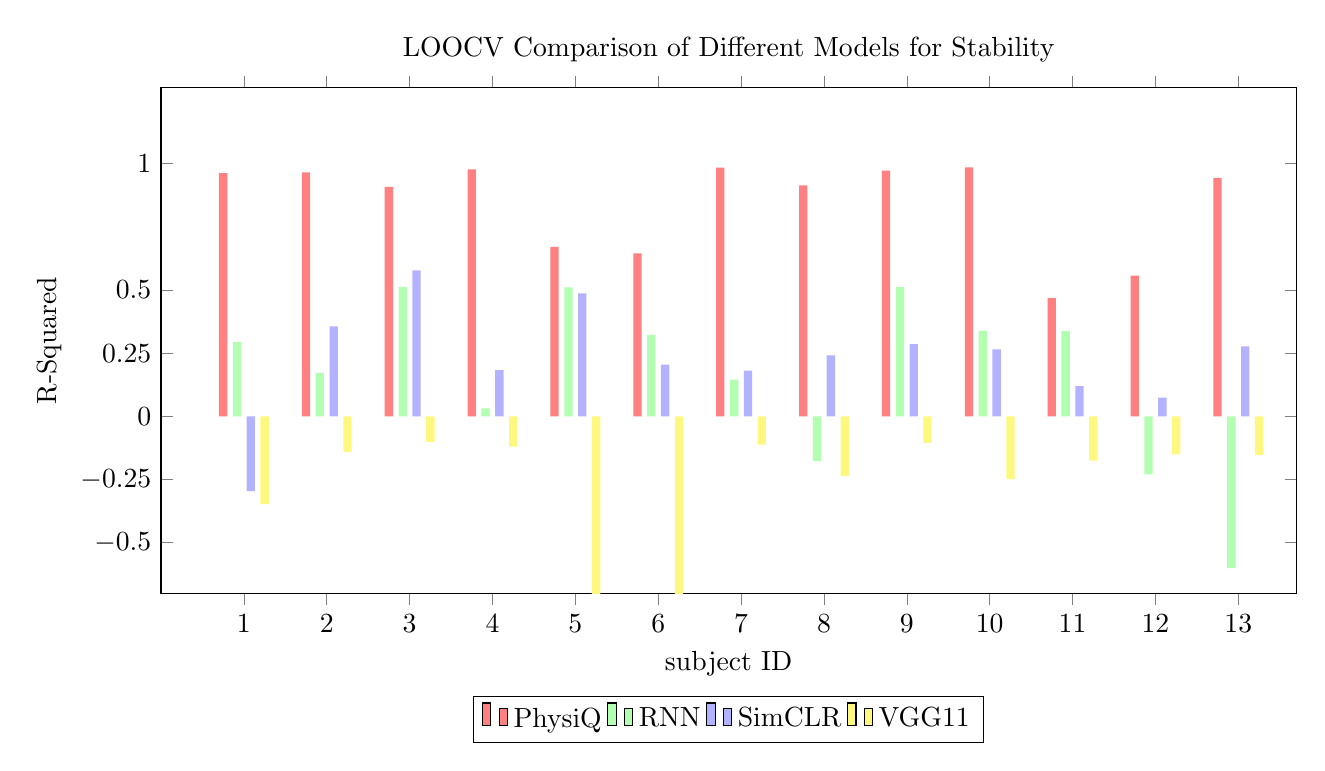
\begin{tikzpicture}
\begin{axis}[
    ybar,
    title=LOOCV Comparison of Different Models for Stability,
% 	x tick label style={
% 		/pgf/number format/1000 sep=},
	xlabel=subject ID,
	ylabel=R-Squared,
xtick={1,2,3,4,5,6,7,8,9,10,11,12,13},
ytick={-.5,-.25, 0, 0.25,  .5, 1.0},
% axis equal,
bar width=3pt,
height=8cm,width=16cm,
% 	enlargelimits=.1,
xmin=0, xmax=13.7, ymin=-.7, ymax=1.3,
	legend style={at={(0.5,-.25
	)},
	anchor=center,legend columns=-2},
% 	nodes near coords,  
%     nodes near coords align={vertical},  
% 	ybar interval=.4,
]
\addplot[draw=none, fill=red!50]  
%PhysiQ with attention
	coordinates {
	(1, 0.962759)
(2, 0.965883)
(3, 0.908476)
(4, 0.977755)
(5, 0.670809)
(6, 0.645153)
(7, 0.984199)
(8, 0.913709)
(9, 0.972433)
(10, 0.985297)
(11, 0.46807)
(12, 0.557421)
(13, 0.943878)
% python .\siamese_cross_validation.py --exercise sa --metrics stability  --lr .001 --hidden_size 256 --epochs 25 --dropout .2
% \begin{comment}
% average 0.8427571601500191
% (3, 0.962759, 0.00230378)
% (8, 0.965883, 0.0021105)
% (9, 0.908476, 0.00566173)
% (10, 0.977755, 0.00137607)
% (11, 0.670809, 0.020364)
% (12, 0.645153, 0.0219511)
% (13, 0.984199, 0.000977434)
% (14, 0.913709, 0.00533803)
% (15, 0.972433, 0.00170533)
% (16, 0.985297, 0.000909541)
% (17, 0.46807, 0.0329056)
% (18, 0.557421, 0.0273783)
% (19, 0.943878, 0.00347175)
% \end{comment}

};
\addplot[draw=none, fill=green!30]
	coordinates {
(1, 0.294923) 
(2, 0.17256) 
(3, 0.512831) 
(4, 0.0316302) 
(5, 0.510665) 
(6, 0.322193) 
(7, 0.145134) 
(8, -0.177127) 
(9, 0.511648) 
(10, 0.337905) 
(11, 0.337649) 
(12, -0.22917) 
(13, -0.600711) 
};

% average 0.16693313646634234
% (3, 0.294923, 0.0105827) 
% (8, 0.17256, 0.0124193) 
% (9, 0.512831, 0.00731207) 
% (10, 0.0316302, 0.0145346) 
% (11, 0.510665, 0.00734459) 
% (12, 0.322193, 0.0101734) 
% (13, 0.145134, 0.012831) 
% (14, -0.177127, 0.0176679) 
% (15, 0.511648, 0.00732984) 
% (16, 0.337905, 0.0099376) 
% (17, 0.337649, 0.00994145) 
% (18, -0.22917, 0.018449) 
% (19, -0.600711, 0.0240256) 
\addplot[draw=none, fill=blue!30]
	coordinates {
(1, -0.295405) 
(2, 0.356205) 
(3, 0.577606) 
(4, 0.183517) 
(5, 0.486332) 
(6, 0.204654) 
(7, 0.180871) 
(8, 0.241452) 
(9, 0.286067) 
(10, 0.265597) 
(11, 0.119688) 
(12, 0.0739067) 
(13, 0.276641) 
 };
\addplot[draw=none, fill=yellow!50] 
	coordinates {
(1, -0.347592) 
(2, -0.140759) 
(3, -0.101083) 
(4, -0.119998) 
(5, -0.735928) 
(6, -0.872492) 
(7, -0.111727) 
(8, -0.236336) 
(9, -0.104602) 
(10, -0.248734) 
(11, -0.174895) 
(12, -0.150518) 
(13, -0.152214) 
 };
	
\legend{PhysiQ, RNN, SimCLR, VGG11}

\end{axis}
\end{tikzpicture}
\caption{We also show the performance of shoulder abduction with the metrics of \textit{stability}. PhysiQ, shown in red, has perform significantly better than other models.}
\label{fig:stability}
\end{figure}


\subsubsection{Classification}
Next, we evaluate the PhysiQ's classification component on the quality of activity, i.e., how accurate can our model predict on \textit{ROMs}. Thus, our baselines for the models are some of the best classification models that modern machine learning and deep learning can achieve: CNN with Multi-Layer Perceptrons (MLP), LSTM with MLP, and Logistic Regression (Linear). Because classification and similarity comparison are two different problems, we target our problem using a different baseline but similar structure overall. CNN with MLP utilizes the 1-D Convolutional Neural Network to capture spatial knowledge and use the hidden representation to go through an MLP network to classify \textit{ROMs} and \textit{stability}. Similarly, LSTM with MLP has a similar approach, except a sliding windows segmentation is used to create a temporal representation, which feeds into the fully connected layer as MLP. Lastly, Logistic Regression is simply a fully connected model that considers all the points (dimensional flattening) in the signal and predicts the labels.

% \pgfplotsset{width=7cm,compat=1.8}
\begin{figure}
    \centering
    \includegraphics[width=\textwidth]{Data_figures/Figure2.png}
% \begin{tikzpicture}
% \begin{axis}[
%     ybar,
%     title= \change{LOOCV Accuracy  Among Different Models for Classifying Range of Motions Labels},
% % 	x tick label style={
% % 		/pgf/number format/1000 sep=},
% 	xlabel=subject ID,
% 	ylabel=Accuracy Percentage,
% xtick={1,2,3,4,5,6,7,8,9,10,11,12,13,14,15,16,17,18,19,20,21,22,23,24,25,26,27,28,29,30,31},
% ytick={ 0, .25,  .5, 1.0},
% % axis equal,
% bar width=1.5pt,
% height=6cm,width=16cm,
% % 	enlargelimits=.1,
% xmin=0,xmax=31.8, ymin=0, ymax=1,
% 	legend style={at={(0.5,-.35
% 	)},
% 	anchor=center,legend columns=-2},
% % 	nodes near coords,  
% %     nodes near coords align={vertical},  
% % 	ybar interval=.4,
% ]
% \addplot[draw=none, fill=red!55]  
% % python .\classification.py --exercise e1 --metrics rom  --lr .001 --hidden_size 256 --epochs 50 --dropout .2 --filename PHYSIQ_E1
% 	coordinates {
% (1, 0.9)
% (2, 0.98)
% (3, 0.98)
% (4, 0.92)
% (5, 0.92)
% (6, 0.82)
% (7, 0.96)
% (8, 0.94)
% (9, 0.96)
% (10, 0.88)
% (11, 0.9)
% (12, 0.76)
% (13, 0.94)
% (14, 0.98)
% (15, 0.9)
% (16, 0.96)
% (17, 0.88)
% (18, 0.64)
% (19, 0.9)
% (20, 1.0)
% (21, 0.96)
% (22, 0.86)
% (23, 1.0)
% (24, 0.86)
% (25, 0.84)
% (26, 1.0)
% (27, 0.88)
% (28, 0.78)
% (29, 1.0)
% (30, 0.94)
% (31, 0.98)


% };
% % python .\classification.py --exercise e1 --metrics rom  --lr .001 --hidden_size 256 --epochs 50 --dropout .2 --filename BASELINE_LOG_E1 --baseline log

% \addplot[draw=none, fill=green!30]
% 	coordinates {
% (1, 0.22)
% (2, 0.58)
% (3, 0.82)
% (4, 0.96)
% (5, 0.84)
% (6, 0.88)
% (7, 0.56)
% (8, 0.9)
% (9, 0.9)
% (10, 0.7)
% (11, 0.92)
% (12, 0.68)
% (13, 0.68)
% (14, 0.94)
% (15, 0.98)
% (16, 0.7)
% (17, 0.48)
% (18, 0.32)
% (19, 0.82)
% (20, 0.76)
% (21, 0.92)
% (22, 0.6)
% (23, 0.62)
% (24, 0.78)
% (25, 0.64)
% (26, 0.88)
% (27, 1.0)
% (28, 0.58)
% (29, 0.94)
% (30, 0.82)
% (31, 0.8)
% };
% \addplot[draw=none, fill=blue!30]
% coordinates {%python .\classification.py --exercise e1 --metrics rom  --lr .001 --hidden_size 256 --epochs 50 --dropout .2 --filename BASELINE_CNN_E1 --baseline cnn
% (1, 0.34)
% (2, 0.6)
% (3, 0.78)
% (4, 0.84)
% (5, 0.64)
% (6, 0.82)
% (7, 0.48)
% (8, 0.82)
% (9, 0.9)
% (10, 0.66)
% (11, 0.9)
% (12, 0.7)
% (13, 0.62)
% (14, 0.84)
% (15, 0.92)
% (16, 0.62)
% (17, 0.7)
% (18, 0.38)
% (19, 0.8)
% (20, 0.72)
% (21, 0.88)
% (22, 0.5)
% (23, 0.64)
% (24, 0.76)
% (25, 0.6)
% (26, 0.76)
% (27, 0.92)
% (28, 0.54)
% (29, 0.88)
% (30, 0.54)
% (31, 0.68)

%  };
% \addplot[draw=none, fill=yellow!50] 
% 	coordinates {%python .\classification.py --exercise e1 --metrics rom  --lr .001 --hidden_size 256 --epochs 50 --dropout .2 --filename BASELINE_RNN_E1 --baseline rnn
% (1, 0.48)
% (2, 0.58)
% (3, 0.72)
% (4, 0.66)
% (5, 0.62)
% (6, 0.52)
% (7, 0.76)
% (8, 0.36)
% (9, 0.74)
% (10, 0.44)
% (11, 0.56)
% (12, 0.6)
% (13, 0.62)
% (14, 0.8)
% (15, 0.6)
% (16, 0.64)
% (17, 0.52)
% (18, 0.24)
% (19, 0.4)
% (20, 0.8)
% (21, 0.52)
% (22, 0.38)
% (23, 0.56)
% (24, 0.42)
% (25, 0.32)
% (26, 0.68)
% (27, 0.48)
% (28, 0.32)
% (29, 0.32)
% (30, 0.56)
% (31, 0.56)

%  };
	
% \legend{PhysiQ, Logistic Regression, CNN,LSTM}

% \end{axis}
% \end{tikzpicture}
\caption{This figure shows the accuracy of our model with output of classification of \textit{range of motion}. As showed in this figure, our PhysiQ (shown in red) performs mostly better than the other models in this diagrams with a percentage accuracy on y-axis.}
\label{figure:loocv_class}
\end{figure}


As a result, we provide confusion matrices for all baselines and our model for classification of \textit{range of motion}. As shown in Figure   \ref{fig:sa_rom_classification:a}, \ref{fig:er_rom_classification:a}, and \ref{fig:ff_rom_classification:a}, compared against the other 3 baselines, our model demonstrates the best performance overall with a minimal inaccuracy on higher degree \textit{range of motion} exercises. The difficulties in differentiating between 30 and 60 degrees happen because of limited supervision and little self-reflection (such as a mirror), and all subjects might not perform homogeneously in the exercises. As a result, this might leads to inconsistency in the model to understand the difference between 30 degrees and 60 degrees ROM.

% \begin{table}[h!]
% \centering
% \begin{tabular}{||c | c | c | c | c||} 
%  \hline
%  Subject & PhysiQ  & Logistic Reg. & CNN & RNN \\ [0.5ex] 
%  \hline\hline
% 1   & 0.9333     & 0.7333    & 0.8   & 0.6333  \\ 
% 2   & 0.5       & 0.3667    & 0.6   & 0.4667  \\
% 3   & 0.7       & 0.7       & 0.6   & 0.4333  \\
% 4   & 0.6333    & 0.4667    & 0.5667& 0.5333  \\
% 5   & 0.9667    & 0.5667    & 0.7333& 0.6  \\
% 6   & 1.0       & 0.5667    & 0.5333& 0.4333  \\
% 7   & 0.7667    & 0.3333    & 0.7333& 0.4333  \\
% 8   & 0.5       & 0.5       & 0.4   & 0.3333  \\ 
% \hline
% avg & 0.7458    & 0.5292    & 0.6203& 0.4833  \\
%  \hline
% \end{tabular}
% \caption{LOOCV on Exercise External Rotation classification of \textit{range of motion}, with an average of 75\% accuracy on our models \meiyi{baseline?}}
% \label{table:er_class_rom}
% \end{table}
% python .\classification.py --exercise er  --lr .001 --batch_size 64
% percentage: 0.8
% (6, 1.0)
% (7, 0.7)
% (8, 0.733333)
% (9, 0.633333)
% (10, 0.966667)
% (11, 0.966667)
% (12, 0.966667)
% (13, 0.433333)\





% [todo: repetition classification]
% 
\begin{figure}
 \begin{subfigure}{0.24\textwidth}
     \includegraphics[width=\textwidth]{Figures/e1_physiq.png}
     \caption{PhysiQ}
     \label{fig:sa_rom_classification:a}
 \end{subfigure}
 \hfill
 \begin{subfigure}{0.24\textwidth}
     \includegraphics[width=\textwidth]{Figures/e1_baseline_logistic_regression.png}
     \caption{Logistic regression}
     \label{fig:sa_rom_classification:b}
 \end{subfigure}
 \hfill
%  \medskip
 \begin{subfigure}{0.24\textwidth}
     \includegraphics[width=\textwidth]{Figures/e1_baseline_cnn.png}
     \caption{CNN}
     \label{fig:sa_rom_classification:c}
 \end{subfigure}
 \hfill
 \begin{subfigure}{0.24\textwidth}
     \includegraphics[width=\textwidth]{Figures/e1_baseline_lstm.png}
     \caption{RNN}
     \label{fig:sa_rom_classification:d}
 \end{subfigure}

 \caption{This is the confusion matrices for classification of \textit{range of motion} in \textbf{shoulder abduction} with PhysiQ and baselines. Shoulder abduction has class of 5 from 30, 60, 90, 120, and 150, which is labeled from 0 to 4}
 \label{fig:sa_rom_classification}

\end{figure}


\begin{figure}
 \begin{subfigure}{0.24\textwidth}
     \includegraphics[width=\textwidth]{Figures/e2_physiq.png}
     \caption{PhysiQ}
     \label{fig:er_rom_classification:a}
 \end{subfigure}
 \hfill
 \begin{subfigure}{0.24\textwidth}
     \includegraphics[width=\textwidth]{Figures/e2_baseline_logistic_regression.png}
     \caption{Logistic regression}
     \label{fig:er_rom_classification:b}
 \end{subfigure}
 \hfill
%  \medskip
 \begin{subfigure}{0.24\textwidth}
     \includegraphics[width=\textwidth]{Figures/e2_baseline_cnn.png}
     \caption{CNN}
     \label{fig:er_rom_classification:c}
 \end{subfigure}
 \hfill
 \begin{subfigure}{0.24\textwidth}
     \includegraphics[width=\textwidth]{Figures/e2_baseline_rnn.png}
     \caption{RNN}
     \label{fig:er_rom_classification:d}
 \end{subfigure}

 \caption{This is the confusion matrices for classification of \textit{range of motion} in \textbf{external rotation} with PhysiQ and baselines. The external rotation has a class of 3 from 45, 90, and 150, which is labeled from 0 to 2}
 \label{fig:er_rom_classification}

\end{figure}

\begin{figure}
 \begin{subfigure}{0.24\textwidth}
     \includegraphics[width=\textwidth]{Figures/e3_physiq.png}
     \caption{PhysiQ}
     \label{fig:ff_rom_classification:a}
 \end{subfigure}
 \hfill
 \begin{subfigure}{0.24\textwidth}
     \includegraphics[width=\textwidth]{Figures/e3_baseline_logistic_regression.png}
     \caption{Logistic regression}
     \label{fig:ff_rom_classification:b}
 \end{subfigure}
 \hfill
%  \medskip
 \begin{subfigure}{0.24\textwidth}
     \includegraphics[width=\textwidth]{Figures/e3_baseline_cnn.png}
     \caption{CNN}
     \label{fig:ff_rom_classification:c}
 \end{subfigure}
 \hfill
 \begin{subfigure}{0.24\textwidth}
     \includegraphics[width=\textwidth]{Figures/e3_baseline_rnn.png}
     \caption{RNN}
     \label{fig:ff_rom_classification:d}
 \end{subfigure}

 \caption{This is the confusion matrices for classification of \textit{range of motion} in \textbf{forward flexion} with PhysiQ and baselines. Forward flexion has a class of 5 from 30, 60, 90, 120, and 150, which is labeled from 0 to 4}
 \label{fig:ff_rom_classification}

\end{figure}


\subsection{Parameters Evaluation}\label{evaluation:subsec:parameters}
\subsubsection{Sliding Windows}
To evaluate the accuracy of our proper performance, we use different sliding window segmentation of samples to test our model results. We test the performance on leave-one-subject-out cross-validation (LOOCV). By having sliding windows that are 50, 100, and 150. The model decreased its performance when the sliding windows increased while keeping the same step size. Increasing the sliding window size decrease the number of time, or redundancy, for the model to see. Having smaller sliding windows helps the model to understand the quality of exercises. At the same time, as we increase the step size (the size of overlapping), the model also performs better but sees a drop in the testing dataset. An extensive redundancy overfits the training distribution and does not generalize it well. As a result, we choose a sliding window of 50 with a step size of 15 for training, validating, and testing, which alike to our data collection rate of 50 Hz. Having some redundancy helps the model to generalize the relationship between sliding windows.

\subsubsection{Repetition Size}
In repetition size, we have a different size in similarity comparison. We have each ID number of segmented exercises for each subject. Adjacent ID number represents that they can be concatenated together to output different. We use the same number of repetition sizes in training and testing. The model has a slight difference in accuracy (3 - 5 percent) in bigger repetitions as length increases. However, this is also affected by the hyperparameters that we choose. Without changing the step size and window size, the model can still perform well because our model generalizes very well. Moreover, we also see a performance increase when adding dropout regularization deep LSTM network. As a result, the performance of four repetitions becomes 0.921 in the R-Squared correlation.


\subsubsection{Padding}
We also evaluate the effect of front padding and back padding. We hypothesize that there should be no difference between front and back padding. However, when the padding is at the end of the temporal sequence, the model does not learn, resulting in an average R-Squared score of 0. Moreover, the results remain unchanged throughout the epochs. This non-learning behavior happens possibly due to the fact that many of the segments are varied significantly. In that cases, many of the windows remain zero and do not help the model to learn. At the same time, as we attempt the model without padding or minimize the amount of padding, we are facing the issue that the temporal model could cheat the result because there is a correlation between higher \textit{range of motion} exercises and the length of the data. In contrast, lower ROM exercises can have a shorter overall length. This relation could result in an accumulating effect of shortcuts for the deep learning model to learn and cheat. So using constant front padding for all one repetition exercises is consistent and performs similarly in a different number of repetitions.  
% [TODO: Would it be more convincing to have random noises]
% [TODO: Cross Validation on Padding]
\subsection{Ablation Study}\label{evaluation:subsec:ablation}
\subsubsection{Removal of Hidden Representations} 
After removing the \textbf{temporal representation}, LSTM encoder, part of PhysiQ, the model still performs relatively well with an MSE 0.007168, MAE 0.0665, and R-Squared 0.8346 with 256 hidden features. At the same time, we did the same procedure for \textbf{spatial representation}. After removing the CNN encoder from PhysiQ, the model performs relatively well with an MSE 0.00873, MAE 0.063, and 0.8208 in R-Squared with one hidden temporal layer and no dropout regularization. Interestingly, in the usages of both spatial and temporal models, our model can achieve 0.92 R-Squared while removing either of them drops significantly by around 10 percent. The decrease happened due to the reasoning that the signal data contain both spatial and temporal information, and a single model can only capture part of the information with the help of an attention mechanism. 
\subsubsection{Dropout}
% python .\siamese_cross_validation.py --exercise sa --metrics rom --hidden_size 256 --batch_size 1024 --num_layers 1 --dropout 0 --epochs 50 --filename dropout_0_evaluation
Testing the dropout is also essential to see how the model is generalized. This dropout is applied in every layer, including the spatial encoder (CNN) and temporal encoder (LSTM). We used LOOCV to compare our results with 0\%, 20\%, and 50\% dropout rates to see if the difference is significant. We test our model with hidden features of 256 for temporal and spatial encoding, two LSTM layers, 16 heads of attention, and a batch size of 1024. The model should not have a significant difference between 20\% and 50\% but possibly a slight performance boost in 20\% or 50\% compared to 0\%. Our model is meant to generalize well across participants and should not overfit the training distribution; the average result of 0 percent dropout across the participants is 89.66\%. The average result with 20 percent dropout is 89.73\%. The average result with 50 percent dropout is 87.87\%. Interestingly, the 20\% dropout rate generates a slightly better results than 50\%.  This is because 20\% has already created its maximal regularization for the model, and increasing the dropout rate does not benefit from regularization. On the other hand, a much higher dropout rate could result in a higher variance in the model, resulted degradation in performance. Having only a 20\% dropout rate creating the maximum of regularization makes our model more convincing in terms of generalizability. 

\subsubsection{Attention}
We test the importance of attention in our model. Attention is applied to selectively focus on more critical aspects of the input sequence. In our model, attention is a final layer to measure the relationship between each hidden state. With that in mind, we remove the attention layer to compare results in the metrics of the \textit{range of motion} in shoulder abduction, external rotation, and forward flexion. Without the attention layer, the performance of LOOCV in shoulder abduction drops to a 0.892 R-squared correlation from 0.908. On exercise external rotation, the performance of LOOCV drops to a 0.560 R-squared correlation from 0.675. Meanwhile, the performance of LOOCV on forward flexion has an insignificant increase from 0.815 to 0.830. In summary, if the motion data is distinguishable and representative, the attention layer does not have a huge impact. However, when exercise has a limited motion, such as half-half arm span exercise external rotation, the attention layer is more impactful.

% [todo: LSTM with one layer does not apply dropout, change it to two if it is possible?] Yes and better!
% (1, 0.0791741)
% (2, 0.672945)
% (3, 0.647328)
% (4, 0.198096)
% (5, 0.721232)
% (6, 0.707202)
% (7, 0.879687)
% (8, 0.935965)
% (9, 0.740117)
% (10, 0.657246)
% (11, 0.753034)
% (12, 0.852191)
% (13, 0.8029)
% (14, 0.952477)
% (15, 0.765612)
% (16, 0.73964)
% (17, 0.887934)
% (18, 0.923182)
% (19, 0.567274)


% \subsection{A Second Exercise: External Rotation}
% We test the \textit{range of motion} metrics of external rotation exercises to support our model's performance. However, segmenting the exercise repetitions is more difficult because the energy of external rotation is significantly lower than shoulder abduction due to its travel distance. Therefore, we have segmented using different parameters for our energy method; we use [1, 0.2, 1] on the weights, dropping the y-axis' importance in producing the energy and changing $\lambda$ to be 0.7, which means the neighbor energy are weighted less. Unfortunately, due to limited time, we have \change{20} participants for three different sets of exercises (45, 90, and 150 in range of motion) to validate our model's generalizability. Interestingly, adding 20\% percent of dropouts can help generalize the model better in testing. It is because due to the different data distribution, dropout acts as a regularization to help better alleviate covariate shift from the testing data. In addition, we discover that subject 8 has the slowest movement speed compared to all other subjects, which explains why the model does not learn in LOOCV when testing subject 8 because the model has never seen this subject's exercise. For example, subject 8 has around 150 data points (3 seconds) compared to other subjects with only 100 data points (2 seconds) with the same ROM. Therefore, it is likely to become a covariate shift when the model is trained based on the first seven subjects and has not seemed to the distribution of subject 8.

% Moreover, we also test using 70-10-20 normal evaluation to test the overall performance. Overall, in 10 test runs, our result of similarity comparison is \change{0.0117 for MSE, 0.0882 for MAE, and 0.757} for R-Squared. Additionally, we test our model with LOOCV on the classification output of ROM, which resulted in an average of \change{83.860}\% accuracy over all subjects. Interestingly, the classification accuracy generates a similar output compared with the R-Squared similarity comparison, that subject 8 has the lowest prediction accuracy.
% \change{
% \subsection{A Third Exercise: Forward Flexion}
% We test the \textit{range of motion}, \textit{stability}, and \textit{repetitions} metrics of forward flexion exercises to further evaluate our model's performance. In order to segment this exercise, we use slightly different parameters compared to shoulder abduction while they are similar in actions. We segment the data using [1, 0.01, 0.8] on the weights, dropping the y-axis' importance and narrowly alleviating the z-axis, and we change $\lambda$ to be 1, making the neighbor energy to be more vital. 
% We have 12 participants in  forward flexion for five sets  (30, 60, 90, 120, and 150 in the range of motion). IN 70-10-20 for \textit{range of motions}, we have a performance of MSE of 0.00215, MAE of 0.0366, and R2 of 0.950. Similarly, in \textit{stability} we have a performance of MSE of 0.00602307, MAE of 0.0594639, and R2 of 0.883. Additionally, in LOOCV, for \textit{repetitions} of \textit{range of motion}, we have 0.8137, 0.8363, and 0.9018 in repetitions 1, 2, and 3 respectively. Interestingly, forward flexion's performance is slightly better than external rotation. Forward flexion and shoulder abduction are part of half arm span exercises with a greater traveling distance of motion in the arm. However, the external rotation has a smaller distance of motion that might make the model harder to understand the underlying structure through supervised learning.}
% classifcation accuracy:
% percentage: 0.6625
% (6, 0.9)
% (7, 0.4)
% (8, 0.633333)
% (9, 0.633333)
% (10, 0.933333)
% (11, 0.966667)
% (12, 0.6)
% (13, 0.233333)

% \begin{table}[h!]
% \centering
% \begin{tabular}{||c c c||} 
%  \hline
%     Subject & R-Squared & MSE \\  [0.5ex] 
%  \hline\hline
%     1 &     0.68336    & 0.0187787    \\ 
%     2 &     0.226178   & 0.0458925  \\
%     3 &     0.300519   & 0.0414836  \\
%     4 &     0.427823   & 0.0339337  \\
%     5 &     0.792675      & 0.0122956 \\
%     6 &     0.792591     & 0.0123007  \\
%     7 &     0.76821   & 0.0137466  \\
%     8 &     0.192196   & 0.0479078   \\
%  \hline
% \end{tabular}
% \caption{Similarity Comparison Results with External Rotation Data}
% \label{table:ER_crossvalidation_Result}
% \end{table}
% Adam optimizer
% python .\siamese_cross_validation.py --exercise er --lr .001 --dropout .2 -- num_layer 2
% average 0.5229439409029432
% (6, 0.68336, 0.0187787)
% (7, 0.226178, 0.0458925)
% (8, 0.300519, 0.0414836)
% (9, 0.427823, 0.0339337)
% (10, 0.792675, 0.0122956)
% (11, 0.792591, 0.0123007)
% (12, 0.76821, 0.0137466)
% (13, 0.192196, 0.0479078)




% train on one exercise and test on other exercise
% train on 1 repetition and test on more than 1 repetition
% varied length comparison? do we need padding?


%\subsection{Principle Component Analysis (PCA) Visualization of Model Representation}

% PhysiQ 0.00619457 mae 0.0627772 r2 0.85198
% SimQLR mse 0.0104795 mae 0.0785231 r2 0.757808
% VGG contrastive mse 0.0469153 mae 0.179209 r2 -0.0817496

%
% input_size=6, hidden_size=256, num_layers=1, batch_size=256, batch_first=True, attention_flag=True, width=50, step=15, bidirectional=False, num_heads=16, total_length=1550, cnn_kernel_size=3, output_size=5, dropout=0.0, lr=0.0001, epochs=50, decoder_mode='siamese', sub_info=False, test=False, num_reps=5)


% Shoulder abd stability:
% 	- Cross validation table
% 	- 70-10-20 table
	
% External rotation rom:
% 	- Cross validation table
% 	- 70-10-20 table

% MLP:
% Baseline:
% 	- Random Forest
% Different variation:
% 	- CRNN
% 	- CRNN + CNN
% 	- CRNN + CNN + Attention
% Shoulder abd rom:
% 	- Classification confusion matrix
	
	
% Shoulder abd stability: 
% 	- Binary or classification (ROC or confusion matrix)

% External rotation rom:
% 	- Classification confusion matrix

